% Style template ines (july 2015)
\documentclass[ngerman]{zhawines}
%\documentclass[german]{scrreprt}
%\newcommand{\headings}{}
%\newcommand{\email}{}
%\sloppy

% Include
\usepackage[ngerman]{babel}
\usepackage{scrpage2}
\usepackage{listings}
\usepackage{amsmath}
\usepackage[squaren]{SIunits}
\usepackage{graphicx}
\usepackage{array}
\usepackage{todonotes}
\usepackage{float}
\usepackage[toc,page]{appendix}
\usepackage[autostyle=true,german=quotes]{csquotes} % quotes
%\usepackage[latin1]{inputenc}    %Umlaute

%\renewcommand{\contentsname}{Inhaltsverzeichnis}

%---------------------------------------------------------------------
\begin{document}

	\hbadness 10000
	\author{Katrin Bächli }
	\betreuer{Prof. Hans Joachim Gelke }
	\nebenbetreuer{Dr. Matthias Rosenthal }
	\title{PA15\_gelk\_1 Polyphonic DDS Synthesizer mit MIDI Steuerung}
	\subtitle{PA15\_gelk\_1 Polyphonic DDS Synthesizer mit MIDI Steuerung}
	\email{katrin.baechli@zhaw.ch}


	\maketitle
	
	\headings
	
	% Inhaltsverzeichnis	
	\tableofcontents
				
	
	% To Do-Liste 
	\listoftodos     % TO DEL am Ende
	
	
	%%%%%%%%%%%%%%%%%%%%%%%%%%%%%%%%%%%%%%%%%%%%%%%%%%%%%%%%%%%%%%%%%
%  _____       ______   ____									%
% |_   _|     |  ____|/ ____|  Institute of Embedded Systems	%
%   | |  _ __ | |__  | (___    Wireless Group					%
%   | | | '_ \|  __|  \___ \   Zuercher Hochschule Winterthur	%
%  _| |_| | | | |____ ____) |  (University of Applied Sciences)	%
% |_____|_| |_|______|_____/   8401 Winterthur, Switzerland		%
%																%
%%%%%%%%%%%%%%%%%%%%%%%%%%%%%%%%%%%%%%%%%%%%%%%%%%%%%%%%%%%%%%%%%

\chapter{Einleitung}\label{chap.einleitung}
Nennt bestehende Arbeiten zu diesem Thema (Literaturrecherche)

Stand der Technik: Bisherige Lösungen des Problems und deren Grenzen


\section{Ausgangslage}\label{sect.einleitung_ausgangslage}
Für den ersten Teil der Arbeit, die zwei ungewollten Effekte von \textit{glitch} und einem metastabilen Zustand herzustellen gibt es selbsterklärend wenige Referenzprojekte. Beide Zustände sind nicht gewollt und finden als solche wohl oft Erwähnung in der Literatur \cite{ReferenceManual} \cite{F_glitches} \cite{F_metastability}, doch wie man diese Zustände provoziert, scheint bis auf eine gefundene \cite{Metastabil}, nicht von Interesse zu sein.
Aus diesem Grund bestehen die ersten zwei Schritte vorwiegend aus eigenen Überlegungen, bzw. aus der Erfahrung von Prof. Hans-Joachim Gelke und seinen Anregungen.


Im zweiten Teil geht es um den Aufbau eines \textit{midi interfaces}. MIDI bedeutet \textit{musical instrument digital interface} und ist ein Standard, der sowohl die genaue Beschaffenheit der erforderlichen Hardware wie auch das Kommunikationsprotokoll der zu übermittelnden Daten festlegt \cite{Midi_Braut}. Die MIDI Manufacturers Association dokumentiert die mehrfachen Erweitungen des MIDI 1.0 Standard \cite{Midi_specification}. Diese Spezifikationen sind relevant in der Entwicklung des Blocks \textit{midi control}.

Am Institut for Embedded Systems bestand bereits die MIDI UART von Armin Weiss. Diese detektiert die empfangenen Bytes und sendet ein valid-Flag, wenn das Byte korrekt ist. Das Byte wird als logic Vetor übermittelt. In dieser Projektarbeit zu entwickeln sind deshalb die zwei Einheiten \textit{midi control}  und \textit{polyphony out}. Und anschliessend diese Blocks in das bestehende Synthesizer-Projekt einzubauen.


Jeder zu entwickelnde Block wird mit einer textbasierten \textit{testbench} getestet. 

\section{Zielsetzung Aufgabenstellung Anforderungen}\label{sect.einleitung_ziele}
Die offizielle Aufgabenstellung befindet sich im Anhang \ref{chap.anhang_aufgabenstellung} unter ref{sect.aufgabenstellung}. Alle Zitate beziehen sich aus diesem Text.\\

Von Anfang an war die Projektarbeit in zwei Teile geteilt:\\Im ersten Teil sollten "Timing Artifakte demonstriert werden", die zu einem "zu einem vertieften Verständnis der digitalen Design Grundlagen führen." 
Ein Ansatz, wie ein glitch detektiert und ein metastabiler Zustand aufgebaut werden kann ist gegeben:\\
\begin{itemize}
	\item "Erzeugung von Glitches mit einem Zähler und nachgeschaltetem Dekoder. Sichtbarmachung der Glitches mit einem Oszilloskop. Betätigen des asynchronen Resets vom Decoder aus." 

	\item "Provozieren und sichtbarmachung von Metastabilen Zuständen. Hierfür kann z.B. eine Schaltung mit zwei asynchronen externen Takten aufgebaut werden." 
\end{itemize}  

Der Fokus des zweiten Teils liegt im Projektausschrieb bei der Entwicklung vielfälltiger Klangfarben für das Synthesizer-Projekt: \\
"Im zweiten Teil soll mit dem dem Direct Digital Synthesis Verfahren ein Synthesizer mit vielfältigen Klangfarben entwickelt werden. Damit kann anspruchsvolle digitale Schaltungstechnik umgesetzt werden. Zum erreichen der Klangvielfalt können mehrere DDS Generatoren gleichzeitig, mit unterschiedlichen Frequenzen und Phasen betrieben werden. Möglich ist auch eine Frequenzmodulation mit einem zweiten Generator oder Ändern des Volumens mit einer Hüllkurve. \\
Die Ansteuerung soll mit Hilfe eines MIDI Interfaces, welches Polyphonie (mehrere Klaviertasten gleichzeitig gedrückt) unterstützt. Die Implementierung soll im FPGA erfolgen. In der Implementierungsphase der Arbeit soll das Timing der FPGA Implementierung genau betrachtet werden. \\
Am Ende soll eine Referenzimplementierung in Anlehnung an den Yamaha DX7 für das Modul DTP2 entstehen."

Da die Entwicklung des ersten Teils länger dauerte, als vorausgedacht, wurde zu Beginn des zweiten Teils die neuen Anforderungen besprochen, da absehbar wurde, dass alle Anforderungen nicht realistisch sind (siehe Anhang \ref{chap.anhang_aufgabenstellung_neu}) 

Gemäss der Spezifikation des zweiten Teiles sind die nächsten Schritte:
\begin{itemize}
\item "Midi Interface for Keyboard für Polyphonie nach Konzept von gelk\\
o   10 Frequenz Control Ausgänge zur Steuerung der Tonhöhe des Generators\\
o   10 On/Off Ausgänge Ton on/off\\
o   UART wird geliefert von gelk\\
o   VHDL wird von Grund auf neu erstellt.
\item 10 DDS implementieren und mit Mischer Mischen
\item Script basierte Testbench. Testbench erzeugt serielle Midi Daten, so wie sie auf dem DIN Stecker vorkommen (logisch)
\item Testbench liest eine Testscript Datei ein, in welcher die Tastendrücke eines Keyboards abgebildet werden können. Midi Poliphony Spec muss durch die Testbench unterstützt werden können. Velocity muss nicht unterstützt werden."
...
\item "Kein VHDL code ohne Testbench.
\item Block level testbench. Unit Tests."
\end{itemize}
\bigskip
Im Anhang \ref{chap.anhang_hans_midicontrol} und \ref{chap.anhang_hans_polyphonie} finden sich die vorgegebene Umsetzung des \textit{midi interfaces}. Auf der CD befindet sich das Synthesizer-Referenz-Projekt, in welches das \textit{midi interface} eingebaut wird.



		
	%%%%%%%%%%%%%%%%%%%%%%%%%%%%%%%%%%%%%%%%%%%%%%%%%%%%%%%%%%%%%%%%%
%  _____       ______   ____									%
% |_   _|     |  ____|/ ____|  Institute of Embedded Systems	%
%   | |  _ __ | |__  | (___    Wireless Group					%
%   | | | '_ \|  __|  \___ \   Zuercher Hochschule Winterthur	%
%  _| |_| | | | |____ ____) |  (University of Applied Sciences)	%
% |_____|_| |_|______|_____/   8401 Winterthur, Switzerland		%
%																%
%%%%%%%%%%%%%%%%%%%%%%%%%%%%%%%%%%%%%%%%%%%%%%%%%%%%%%%%%%%%%%%%%

\chapter{Glitch}\label{chap.glitch}

\section{Glitch in der Digitalen Signalverarbeitung}\label{sect.glitch_def}
In der Digitalen Signalverarbeitung ist ein \textit{glitch} ein bekanntes, ungewolltes Verhalten, das William I. Fletscher folgendermassen beschreibt:

\begin{quote}
''Als \textit{glitch}  wird eine ungewollte, flüchtige ''Signalspitze'' bezeichnet, die Zähler aufwärts zählt, Register löscht oder einen ungewollten Prozess startet.'' \cite{F_glitches}
\end{quote}


Abbildung \ref{fig.glitch.def} zeigt zwei \textit{glitches} in einem Ausgangssignal.

\begin{figure}[H]
	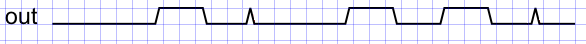
\includegraphics[width=\textwidth]{images/glitch/def_glitch_1.png}
	\caption{Zwei Glitches im Ausgangssignal}
	\label{fig.glitch.def}
\end{figure}


\section{Ursache für Glitches}\label{sect.glitch_ursache}

Der Auslöser sind ungleichzeitig eintreffende Signale, die durch

\begin{enumerate}
\item unterschiedlich lange Signalpfade,
\item unterschiedliche Durchlaufverzögerungen der vorangehenden Flip-Flops oder
\item unterschiedliche Logik-Zeiten
\end{enumerate}

entstehen, und die in ein asynchrones Bauteil geführt werden. Der Dekoder im asynchronen Bauteil entschlüsselt dadurch kurzfristig einen falschen Wert.

Abbildung \ref{fig.glitch.bild1} zeigt ein leicht verzögertes enable-Signal (ena) zu einem anders verzögerten Flip-Flop-Eingangssignal (Q). Beide Signale sind mit der Taktfrequenz clk getaktet. Der Ausgang (out) des Flip-Flops weist aufgrund der unterschiedlichen Verzögerungen kurzzeitig \textit{glitches} auf. \\
\begin{figure}[H]
	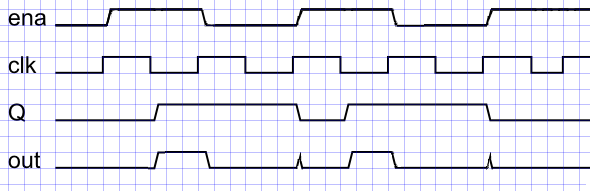
\includegraphics[width=0.8\textwidth]{images/glitch/def_glitch_3.png}
	\caption{Asynchrone Eingangssignale führen zu Glitches}
	\label{fig.glitch.bild1}
\end{figure}


\newpage
\section{Glitch erzeugen}\label{sect.glitch_detect}


\subsection{Konzept}
Glitches werden durch Pfadverlängerung einzelner Werte erzeugt. Ein asynchroner Zähler erhält verzögerte Bitwerte. Zählt man binär auf 15, so kann sich beim Übergang von der Zahl 11 zu 12, die falsche Zahl 15, ergeben, sofern die zwei höheren Bits der Zahl 11 verzögert ankommen (siehe Abbildung \ref {fig.glitch.binaer_zahlen}).

\begin{figure}[H]
	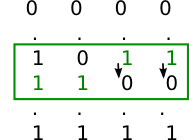
\includegraphics[width=0.3\textwidth]{images/glitch/konzept_verzoegerung.png}
	\caption{Binärwerte des asynchronen Zählers}
	\label{fig.glitch.binaer_zahlen}
\end{figure}

Die Verzögerung der zwei Bits, wird über Routing umgesetzt. 

\subsection{Implementation} 

Die Hardware ist das Altera Board De2 mit dem FPGA Cyclone II. Kompiliert wird das Projekt mit Quartus 13.0sp, der ältesten Quartus-Version, die den Cyclone II unterstützt.

Die Pfad\textit{verlängerung} wird über das Routing über die GPIO-Pins des Stecker 1 gemacht (siehe Abbildung \ref{fig.glitch.GPIO}. GPIO 1 ist der Stecker 1). Dekodiert die asynchrone Logik die Zahl 15, wird das  Reset-Signal (aus der Logik \lstinline|reset_counter\~{}2|) an den Zähler gesendet und der Zähler beginnt wieder von 0 an zu zählen. Produziert der Dekoder zur falschen Zeit einen Reset, so ist dies eine Fehlkodierung: ein \textit{glitch}.

Das RTL-Diagramm des asynchronen Zählers sieht wie folgt aus:
\begin{figure}[H]
	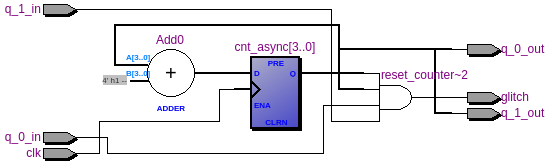
\includegraphics[width=1\textwidth]{images/glitch/RTL_asynchron.png}
	\caption{Asynchroner Zähler mit Routing erzeugt Glitch}
	\label{fig.glitch.RTL_nurGlitch}
\end{figure}

Um die Lösung gegen \textit{glitches} aufzuzeigen, wird dem asynchronen Zähler zur Synchronisation ein Flip-Flop nachgeschalten. Dadurch werden die asynchronen Zustände übersehen. 
\begin{figure}[H]
	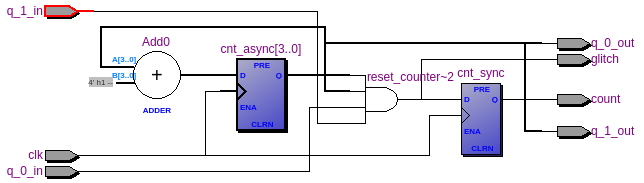
\includegraphics[width=\textwidth]{images/glitch/glitch_asynch_new.png}
	\caption{Glitch-Zähler und synchroner Zähler dazu}
	\label{fig.glitch.RTL_mit_synchr.Zaehler}
\end{figure}

Die Reset-Signale aus der Vergleichslogik (\lstinline|reset_counter\~{}2|) des asynchronen Zählers wie die des synchronisierten Zählers werden an die GPIO Steckers ausgegeben, ebenso der Systemtakt. In der Abbildung \ref{fig.glitch.GPIO}) wird das Signal des asynchronen Zählers als Glitch und das Signal des synchronisierten Zählers als Count benannt. In der GPIO-Pinbelegung sieht man auch die Nutzung der zwei oberen Pin-Reihen für das Routing (benannt mit Routing OUT, IN). Der Systemtakt wird als CLK ausgegeben.

\begin{figure}[H]
	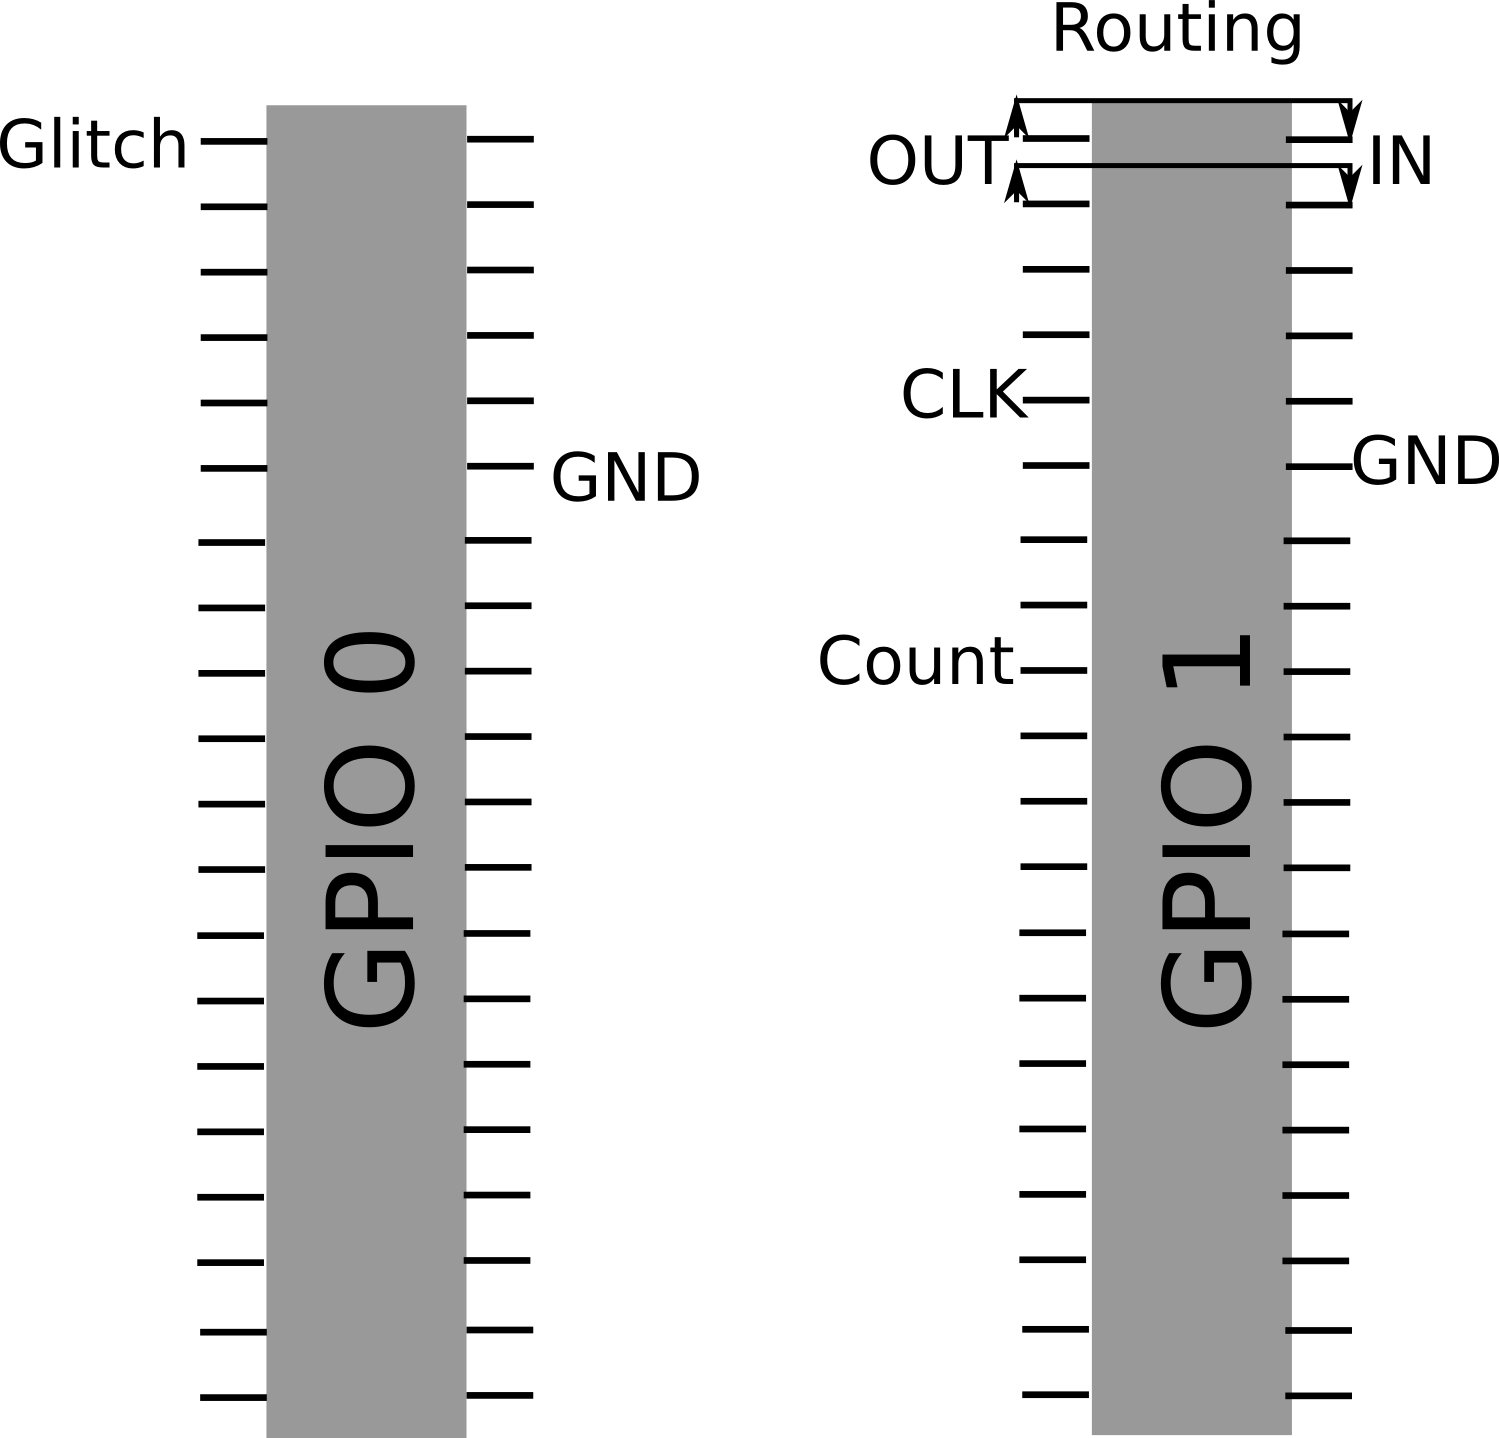
\includegraphics[width=0.5\textwidth]{images/glitch/GPIO_Belegung.png}
	\caption{GPIO Anschlüsse}
	\label{fig.glitch.GPIO}
\end{figure}


\newpage
\section{Resultat }\label{sect.glitch_resultat}

Der Reset des asynchronen Zählers (CH 1), der synchronisierte Reset (CH 2) und der Systemtakt (CH 3) werden am KO ausgegeben. Durch die Synchronisation wird der Wert um 1 Periode (= 20 ns) verzögert.

\begin{figure}[H]
	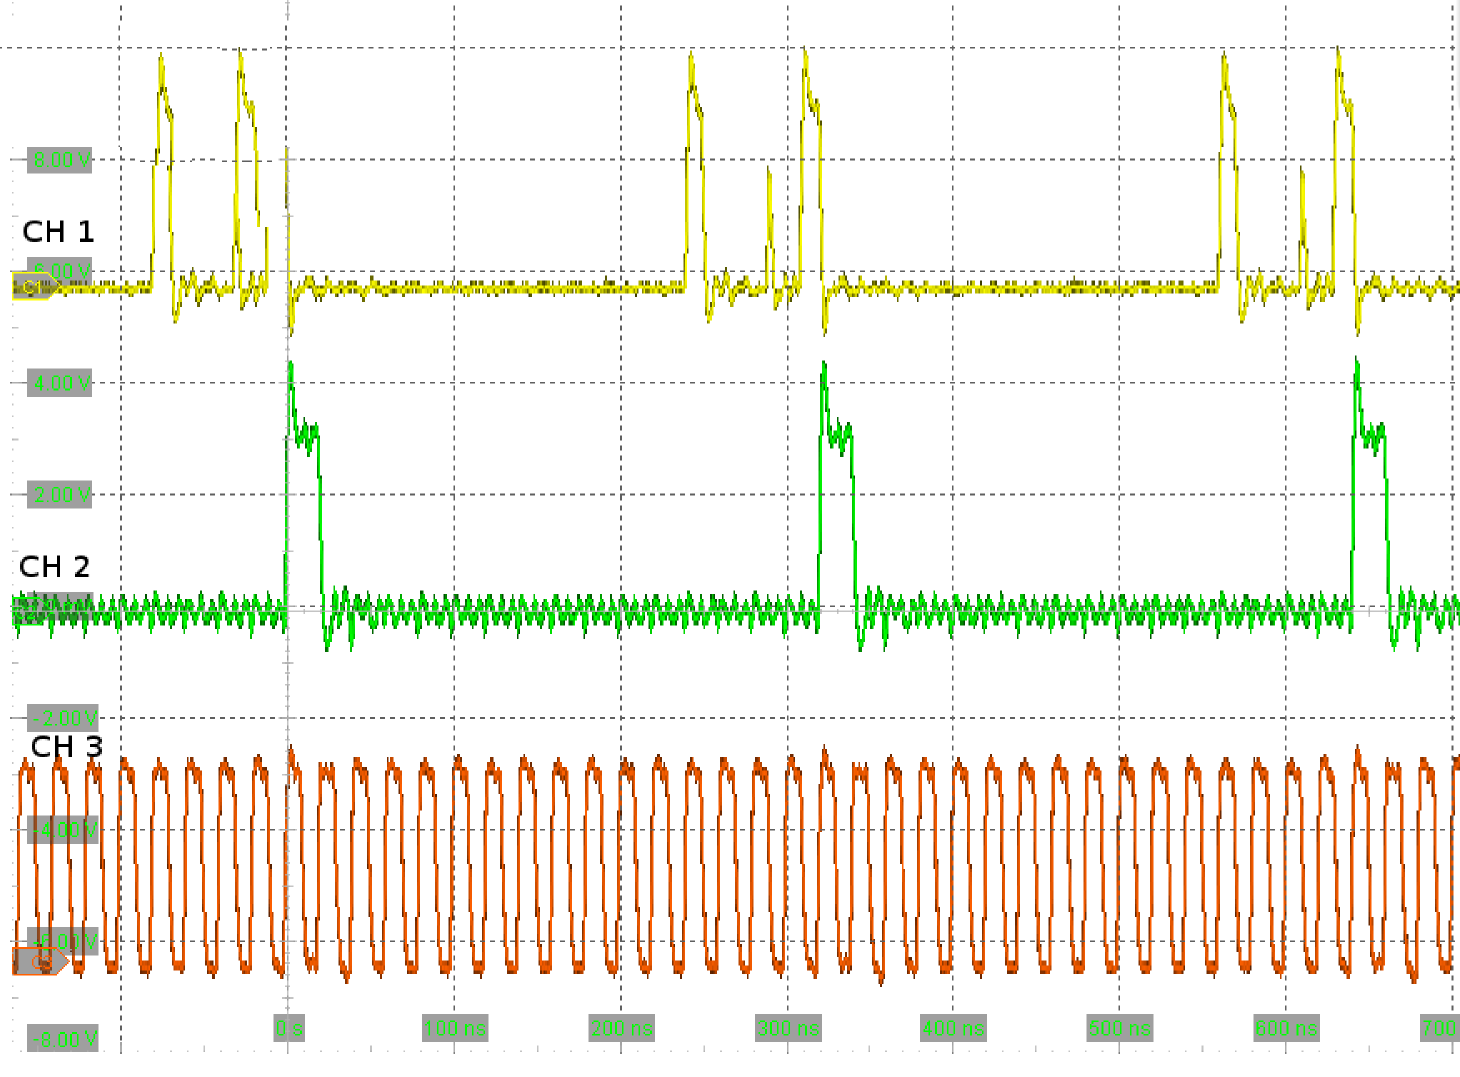
\includegraphics[width=0.6\textwidth]{images/glitch/Glitch_2_good.png}
	\caption{Glitch (gelb), Zähler (grün) und Takt (orange)}
	\label{fig.glitch.result_1}
\end{figure}

 Das \textit{glitch} trifft in der im Übergang von der 11 zur 12 Periode (nach 240 ns) regelmässig auf. Dies ist das zu erwartende Ergebnis. Ein kurzzeitiges asynchrones Verhalten findet sich auch im Übergang von der 13 zur 14 Periode. Dies ist wenn der binäre Wert 1101 auf 1110 wechselt. Da die zwei niederwertigen Bits verzögert sind, ist das Dekodieren des Wertes 1111 plausibel.\\
 
\begin{figure}[H]
	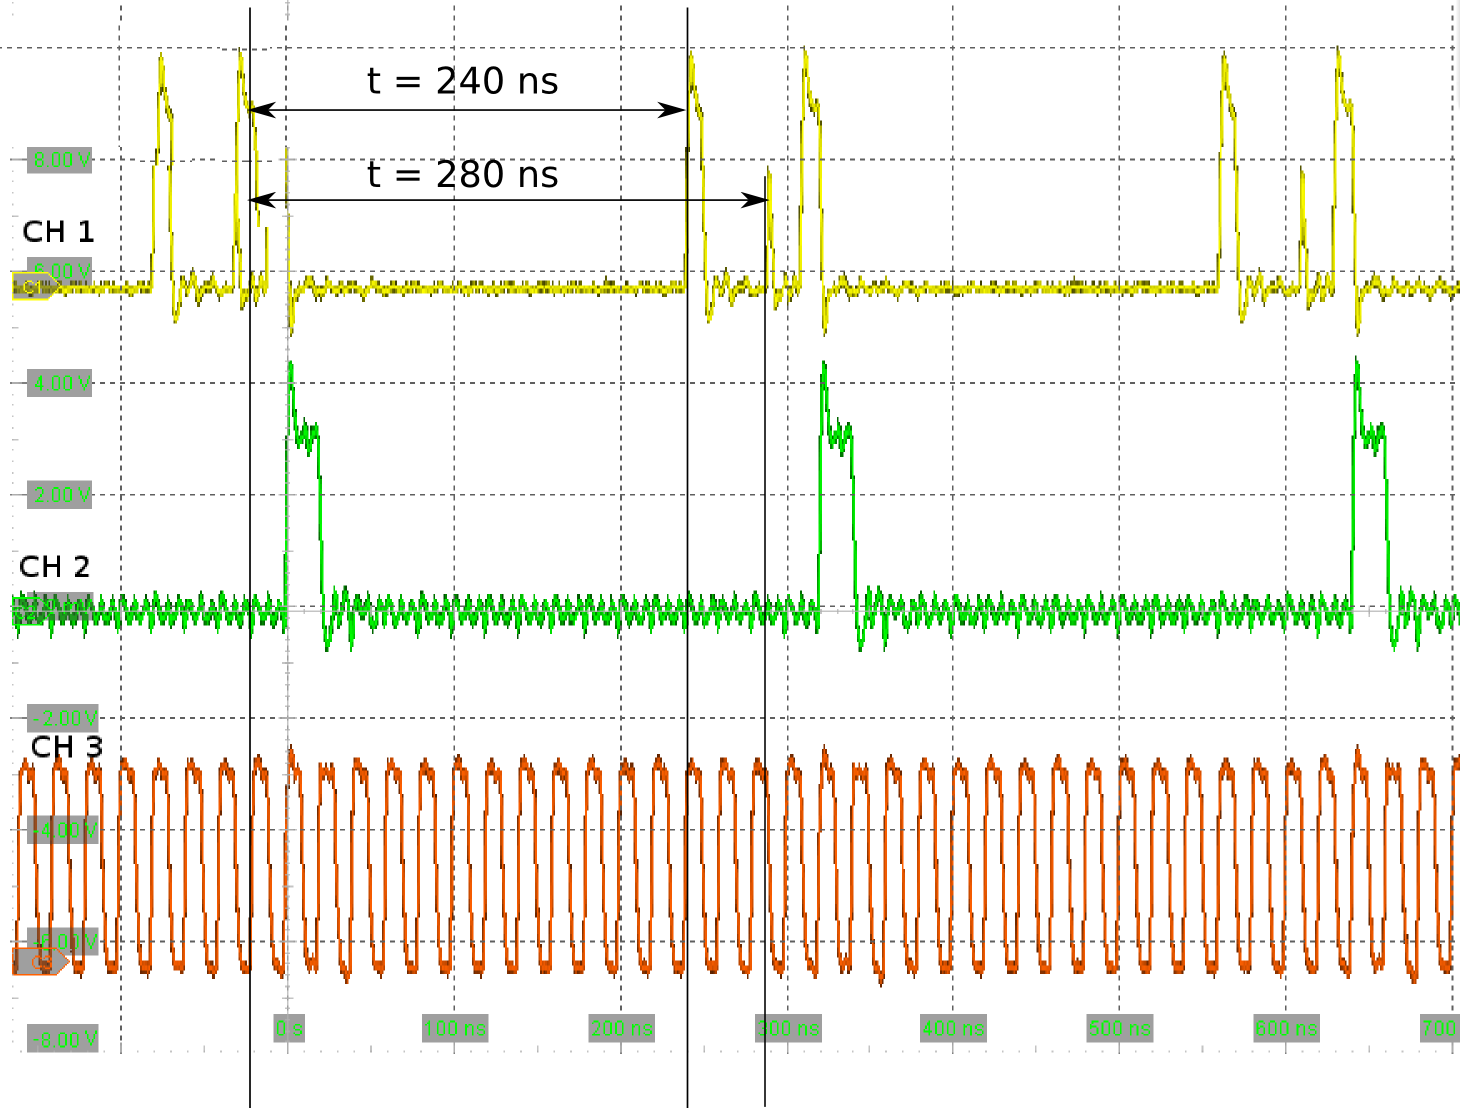
\includegraphics[width=0.6\textwidth]{images/glitch/Glitch_2_timing.png}
	\caption{Zeitanalyse Glitches}
	\label{fig.glitch.result_2}
\end{figure}



 	
	%%%%%%%%%%%%%%%%%%%%%%%%%%%%%%%%%%%%%%%%%%%%%%%%%%%%%%%%%%%%%%%%%
%  _____       ______   ____									%
% |_   _|     |  ____|/ ____|  Institute of Embedded Systems	%
%   | |  _ __ | |__  | (___    Wireless Group					%
%   | | | '_ \|  __|  \___ \   Zuercher Hochschule Winterthur	%
%  _| |_| | | | |____ ____) |  (University of Applied Sciences)	%
% |_____|_| |_|______|_____/   8401 Winterthur, Switzerland		%
%																%
%%%%%%%%%%%%%%%%%%%%%%%%%%%%%%%%%%%%%%%%%%%%%%%%%%%%%%%%%%%%%%%%%

\chapter{Metastabilität}\label{chap.metastabilitat}

\section{Definition Metastabilität}\label{sect.meatastabil_def}
Metastabilität bedeutet, dass der Ausgang eines Flip-Flops nicht dem Eingang entsprechen muss. Wechselt das Inputsignal eines Flip-Flops zur falschen Zeit, ist der Wert des Ausgangssignal unsicher. Hier zwei kurze englische Beschreibungen, dieses Phänomens:\\
\newline
'' If data inputs to a flip-flop are changing at the instant of the clock pulse, a problem known as \textit{metastability} may occur. In the metastable case, the flip-flop does not settle in to a stable state'' (Camara, S. 32-2)  \\
\newline
''If the amplitude of the runt pulse is \textit{exactly the treshold level of the SET input of the output cell}, the cell will be driven to its metastable state. The metastable state is the condition that is roughly defined as ''half SET and half RESET'' (Fletcher, 482.)\\
\newline
\\
Im besten Fall wählt der Ausgang bei unklarem Eingangssingal selbst einen Wert an ('0' oder '1'). Im schlechten Fall “hängt” sich das Flip-Flop “auf” und toggelt permanent zwischen '0' und '1' oder setzt sogar beide Werte parallel.

\begin{figure}[H]
	\centering
	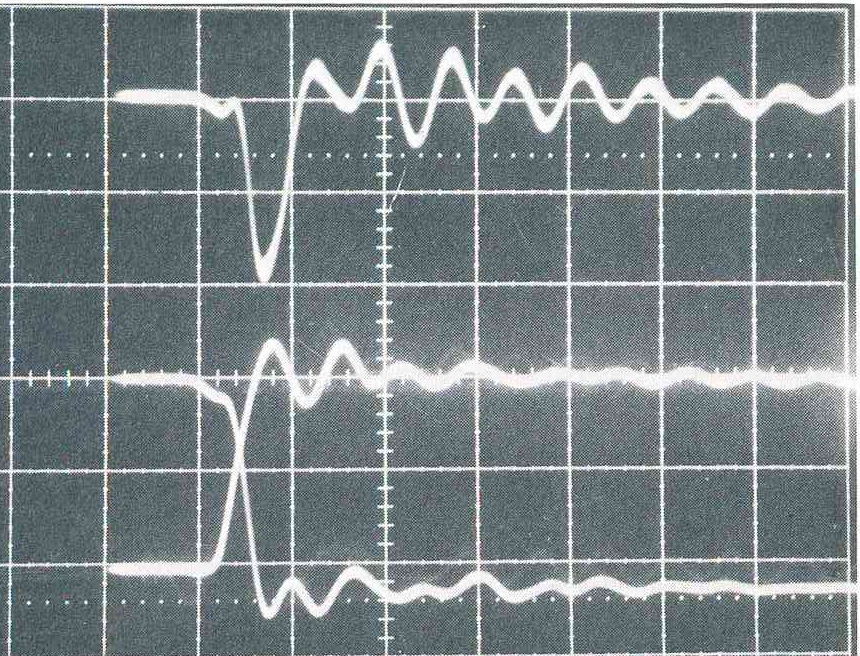
\includegraphics[width=0.4\textwidth]{images/metastability/metastability_2_IO.png}
	\caption{Metastabilität schlimmster Fall (Fletcher, 482.)}
	\label{fig.metastabil.schlimmster_Fall}
\end{figure}


\section{Ursache von Metastabilität}\label{sect.meatastabil_ursache}
Der Grund für Metastabilität ist, dass der angelgte Wert entweder zu spät eintrifft (verletzen der setup-Zeit) oder zu früh wieder verschwindet (verletzen der hold-Zeit). Metastabilität kann vermieden werden, wenn diese zwei Zeiten strikt eingehalten werden:\\
\newline
''Metastabilit is avoided by holding the information stable before and after the clock pulse  for a set period of time, called the setup time for the data line an the hold time for the control line.''(Camara, S. 32-2)
\begin{figure}[H]
	\centering
	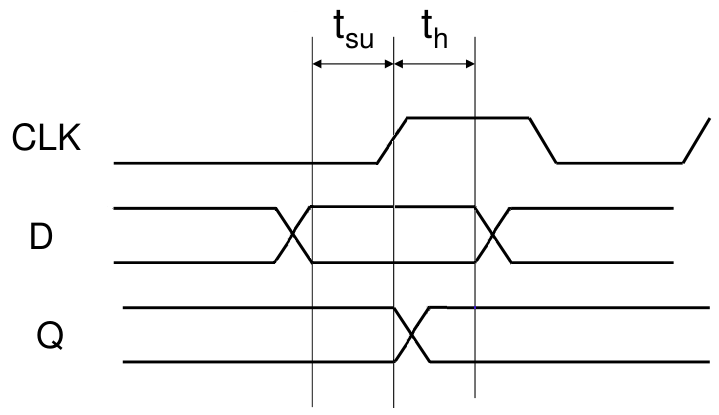
\includegraphics[width=0.4\textwidth]{images/metastability/kritscheZeit_FF.png}
	\caption{Einhalten der Datenzeiten}
	\label{fig.metastabil.kritisches_zeitfenster}
\end{figure}
Es gibt mehrere Gründe für das Nichteinhalten der geforderten setup-Zeit:\\
- Ein Logikpfad kann zu lange sein, bzw. die Taktfrequenz ist zu schnell\\
- Zwischen den Bauteilen liegen zu lange Pfade, die das Eintreffen der Daten verzögern\\
- Ein vorangehendes Bauteil hat eine zu lange Durchlaufverzögerung.\\
\\
Um Metastabilität zu vermeiden, sollte die Logik möglichst klein gehalten werden, die Bauteile bewusst nahe beieinander platziert und vor allem der Systemtakt an die längste Pfadzeit angepasst werden. Der maximal elaubte Systemtakt kann in quartus mit dem Timequest Time Analyser abgefragt werden.\\
Als Alternative bietet sich eine Synchronisierungsschaltung an. Zwischen den zwei Takt-Flanken kann sich der metastabile Ausgang erholen und gelangt so stabil in den Verarbeitungspfad. Der Nachteil der Synchronistation ist jedoch, eine um einen Takt längere Verarbeitungszeit.\\


\section{Metastabilität erzeugen}\label{sect.meatastabil_erzeugen}
\subsection{Ansatz}\label{sect.metastabil_ansatz}
Aufgebaut wird ein System mit zwei Takten. Der zentrale Block hat eine Taktfrequenz von 50 MHz und beinhaltet eine State Machine. Diese wechselt bei jedem Impuls von einem Zustand in den anderen (Abbild: \ref{fig.metastabil.statemachine} Um die zwei Zustände zu erkennen, werden beiden Zuständen ein logischer Pegel zugefügt:\\
\newline
- Zustand 1:  s0  = Logisch '0'\\
- Zustand 2:  s1  = Logisch '1'\\

\begin{figure}[H]
	\centering
	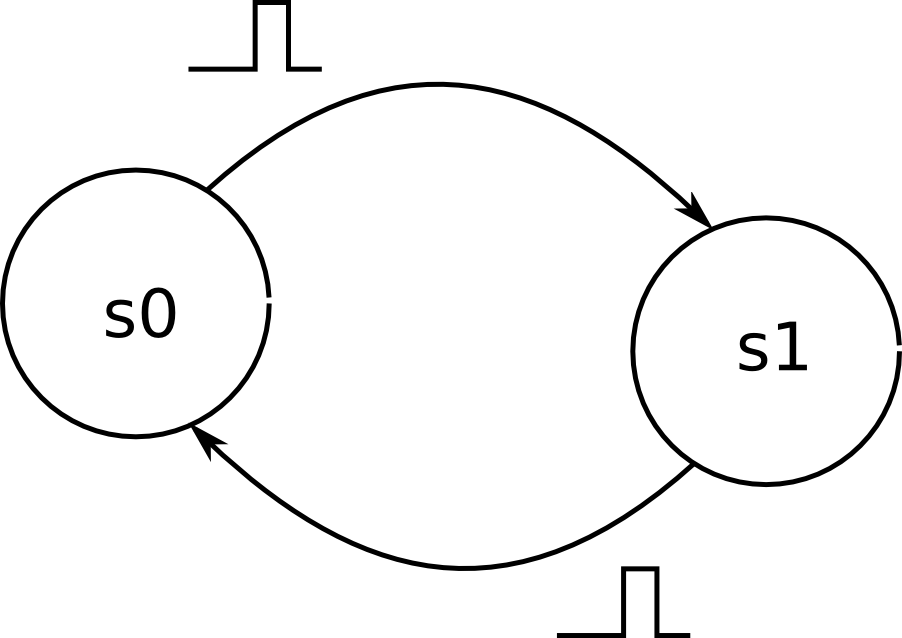
\includegraphics[width=0.2\textwidth]{images/metastability/statemachine_s0_s1.png}
	\caption{Statemachine im zentralen Block}
	\label{fig.metastabil.statemachine}
\end{figure}

Der Inpuls, der die Statemachine steuert ist asynchron. Er wird von einem Zähler generiert, der mit der Taktfrequenz von 27 MHz läuft. Alle 37 ns sendet der Zähler einen Puls an die State Machine. Die State Machine selbst arbeitet mit einer Taktfrequenz von 20 ns. Der Impuls ist ihr gegenüber asynchron.\\
\newline
Erwartet wird, dass die setup-Zeit der State Machine-Flip-Flops regelmässig verletzt werden. \\

\begin{figure}[H]
	\centering
	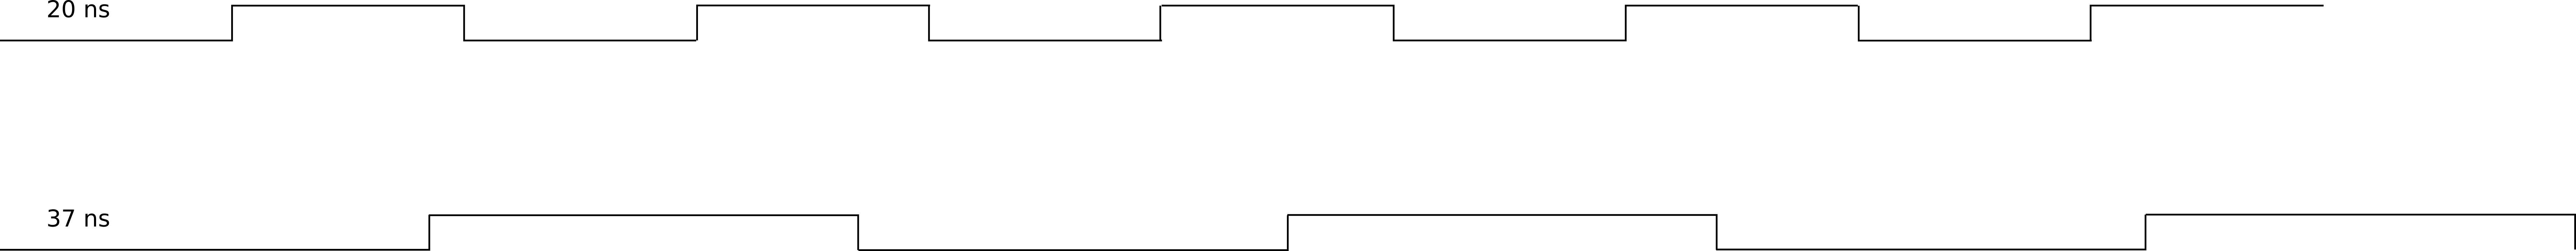
\includegraphics[width=0.2\textwidth]{images/metastability/2_takte.png}
	\caption{Die zwei Taktzeiten}
	\label{fig.metastabil.statemachine}
\end{figure}
\todo{ einsetzen setup zeit gemäss glossar für ..}


\subsection{Implementation}\label{sect.metastabil_implementation}


\section{Resultat Metastabilität provozieren}\label{sect.meatastabil_proozieren}
\textbf{Was ist das Ergebnis beim Verletzen der setup Zeit?}
Beide Ausgänge immer an?
Keiner von beiden?
aufhängen des Systems? (Keine LED geht mehr).

\textbf{Synchronisation Schaltung erhärtet die These b\\}
 				
	%%%%%%%%%%%%%%%%%%%%%%%%%%%%%%%%%%%%%%%%%%%%%%%%%%%%%%%%%%%%%%%%%%
%  _____       ______   ____									%
% |_   _|     |  ____|/ ____|  Institute of Embedded Systems	%
%   | |  _ __ | |__  | (___    Wireless Group					%
%   | | | '_ \|  __|  \___ \   Zuercher Hochschule Winterthur	%
%  _| |_| | | | |____ ____) |  (University of Applied Sciences)	%
% |_____|_| |_|______|_____/   8401 Winterthur, Switzerland		%
%																%
%%%%%%%%%%%%%%%%%%%%%%%%%%%%%%%%%%%%%%%%%%%%%%%%%%%%%%%%%%%%%%%%%

\chapter{Projekt Synthesizers}\label{chap.syntehsizer_projekt}

\section{Vorwissen aus DTP 2}\label{sect.synthesizer_dtp2}


\begin{figure}[H]
	\centering
	
\includegraphics[width=\textwidth]{images/idle.png}
	\caption{Bildbeschreibung ....}
	\label{fig.synthesizer_}
\end{figure}

\subsection{Bauteile De2-115}\label{sect.synthesizer_dtp2_DE2115}
\subsection{Aufbau Synthesizer}\label{sect.synthesizer_dtp2_DE2115}
\subsection{Implementation}\label{sect.synthesizer_dtp2_DE2115}

\section{Neue Bauteile}\label{sect.synthesizer_neues}
\subsection{Steuerung per Handy über Bluetooth}\label{sect.synthesizer_neues_bluetooth}
\subsection{Neue Frequenzmodulation}\label{sect.synthesizer_neues_FM}

 	
	%%%%%%%%%%%%%%%%%%%%%%%%%%%%%%%%%%%%%%%%%%%%%%%%%%%%%%%%%%%%%%%%%%
%  _____       ______   ____									%
% |_   _|     |  ____|/ ____|  Institute of Embedded Systems	%
%   | |  _ __ | |__  | (___    Wireless Group					%
%   | | | '_ \|  __|  \___ \   Zuercher Hochschule Winterthur	%
%  _| |_| | | | |____ ____) |  (University of Applied Sciences)	%
% |_____|_| |_|______|_____/   8401 Winterthur, Switzerland		%
%																%
%%%%%%%%%%%%%%%%%%%%%%%%%%%%%%%%%%%%%%%%%%%%%%%%%%%%%%%%%%%%%%%%%

\chapter{Bluetooth Handy-Ansteuerung}\label{chap.bluetooth}

\section{Bluetooth Modul ZSN}\label{sect.bluetooth_modul}

\begin{figure}[H]
	\centering
	
\includegraphics[width=0.5\textwidth]{images/idle.png}
	\caption{blabla}
	\label{fig.bluetooth_}
\end{figure}


\section{Anbindung in VHDL}\label{sect.bluetooth_vhdl}



\section{Steuerung auf Handy}\label{sect.bluetooth_handy}	
	%%%%%%%%%%%%%%%%%%%%%%%%%%%%%%%%%%%%%%%%%%%%%%%%%%%%%%%%%%%%%%%%%%
%  _____       ______   ____									%
% |_   _|     |  ____|/ ____|  Institute of Embedded Systems	%
%   | |  _ __ | |__  | (___    Wireless Group					%
%   | | | '_ \|  __|  \___ \   Zuercher Hochschule Winterthur	%
%  _| |_| | | | |____ ____) |  (University of Applied Sciences)	%
% |_____|_| |_|______|_____/   8401 Winterthur, Switzerland		%
%																%
%%%%%%%%%%%%%%%%%%%%%%%%%%%%%%%%%%%%%%%%%%%%%%%%%%%%%%%%%%%%%%%%%

\chapter{Frequenzmodultion}\label{chap.frequenzmodulation}

\begin{figure}[H]
	\centering
	
\includegraphics[width=\textwidth]{images/idle.png}
	\caption{Bildbeschreibung ....}
	\label{fig.fm_}
\end{figure}

\subsection{Definition Frequenzmodualtion}\label{sect.fm_definition}

\subsection{Frequenzmodualtion DTP2}\label{sect.fm_DTP2}


\subsection{Frequenzmodualtion neu}\label{sect.fm_neu}
\subsubsection{Ansatz}\label{sect.fm_neu.ansatz}
\subsubsection{Implementation}\label{sect.fm_neu.implementation}
\subsubsection{Resultat}\label{sect.fm_neu.resultat}
	%%%%%%%%%%%%%%%%%%%%%%%%%%%%%%%%%%%%%%%%%%%%%%%%%%%%%%%%%%%%%%%%%%
%  _____       ______   ____									%
% |_   _|     |  ____|/ ____|  Institute of Embedded Systems	%
%   | |  _ __ | |__  | (___    Wireless Group					%
%   | | | '_ \|  __|  \___ \   Zuercher Hochschule Winterthur	%
%  _| |_| | | | |____ ____) |  (University of Applied Sciences)	%
% |_____|_| |_|______|_____/   8401 Winterthur, Switzerland		%
%																%
%%%%%%%%%%%%%%%%%%%%%%%%%%%%%%%%%%%%%%%%%%%%%%%%%%%%%%%%%%%%%%%%%

\chapter{Resultate der Projektarbeit}\label{chap.resultate}



\section{Vertiefung VHDL}\label{sect.resultatePA}
Beides erreicht. Viel Aufwand, da wenig Wissen wie ungewollter Zustand erzeugt werden kann.
Es dauerte 4 Wochen (15. oktober + Doku), der insgesammt 16 Wochen PA.

\section{Synthesizer mit MIDI-Ansteuerung}\label{sect.resultatePA}



	%%%%%%%%%%%%%%%%%%%%%%%%%%%%%%%%%%%%%%%%%%%%%%%%%%%%%%%%%%%%%%%%%
%  _____       ______   ____									%
% |_   _|     |  ____|/ ____|  Institute of Embedded Systems	%
%   | |  _ __ | |__  | (___    Wireless Group					%
%   | | | '_ \|  __|  \___ \   Zuercher Hochschule Winterthur	%
%  _| |_| | | | |____ ____) |  (University of Applied Sciences)	%
% |_____|_| |_|______|_____/   8401 Winterthur, Switzerland		%
%																%
%%%%%%%%%%%%%%%%%%%%%%%%%%%%%%%%%%%%%%%%%%%%%%%%%%%%%%%%%%%%%%%%%

\chapter*{Glossar}\label{chap.glossar}




\textbf{Durchlaufverzögerung}\\
Wird englisch \textit{propagation delay} genannt und bezeichnet die Zeit, die Daten vom Eingang bis zum Ausgang des Bauteils brauchen.\\
Die Durchlaufverzögerung beträgt beim Cylone IV 4 ns (Device Handbook, S. 8-19).\\


\textbf{hold time}\\
Ist die minimale Zeit, in der die Inputdaten \textit{nach} der Taktflanke stabil sein müssen.\\
Die hold-Zeit beträgt beim  Cyclone IV E 0 ns (Device Handbook, S. 8-19).\\


Pfadzeit\\
... (Unter 3.2. Metastabilität Ratschläge erwähnt)\\



\textbf{quartus}\\
IDE von altera zum Kompilieren, Synthesizieren und einbauen von IPs für die altera FPGAs.\\


\textbf{setup time} \\
minimale Zeit, in der Inputdaten stabil sein müssen be\textit{vor} ein Taktflanke die Daten triggert.\\
Die setup-Zeit beträgt beim Cyclone IV E 10 ns (Device Handbook, S. 8-19)\\





	%%%%%%%%%%%%%%%%%%%%%%%%%%%%%%%%%%%%%%%%%%%%%%%%%%%%%%%%%%%%%%%%%%
%  _____       ______   ____									%
% |_   _|     |  ____|/ ____|  Institute of Embedded Systems	%
%   | |  _ __ | |__  | (___    Wireless Group					%
%   | | | '_ \|  __|  \___ \   Zuercher Hochschule Winterthur	%
%  _| |_| | | | |____ ____) |  (University of Applied Sciences)	%
% |_____|_| |_|______|_____/   8401 Winterthur, Switzerland		%
%																%
%%%%%%%%%%%%%%%%%%%%%%%%%%%%%%%%%%%%%%%%%%%%%%%%%%%%%%%%%%%%%%%%%

\pagenumbering{Roman}

\appendix

\chapter{Offizielle Aufgabenstellung}\label{chap.anhang_aufgabenstellung}

\section*{Beschreibung der Projektarbeit PA15\_gelk\_1}\label{sect.aufgabenstellung}

In dieser Projektarbeit sollen Versuche entwickelt werden, die für das Modul DTP2 verwendet werden können. Die Arbeit besteht aus zwei Teilen:

Im ersten Teil der Arbeit sollen Versuche entwickelt werden, mit denen folgende Timing Artefakte demonstriert werden können. Dies soll zum zu einem vertieften Verständnis der digitalen Design Grundlagen führen.

\begin{itemize}
	\item Erzeugung von Glitches mit einem Zähler und nachgeschaltetem Dekoder. Sichtbarmachung der Glitches mit einem Oszilloskop. Betätigen des asynchronen Resets vom Decoder aus. 

	\item Provozieren und Sichtbarmachung von Metastabilen Zuständen. Hierfür kann z.B. eine Schaltung mit zwei asynchronen externen Takten aufgebaut werden. 
\end{itemize}

Im zweiten Teil soll mit dem dem Direct Digital Synthesis Verfahren ein Synthesizer mit vielfältigen Klangfarben entwickelt werden. Damit kann anspruchsvolle digitale Schaltungstechnik umgesetzt werden. Zum erreichen der Klangvielfalt können mehrere DDS Generatoren gleichzeitig, mit unterschiedlichen Frequenzen und Phasen betrieben werden. Möglich ist auch eine Frequenzmodulation mit einem zweiten Generator oder Ändern des Volumens mit einer Hüllkurve. Die Ansteuerung soll mit Hilfe eines MIDI Interfaces, welches Polyphonie (mehrere Klaviertasten gleichzeitig gedrückt) unterstützt. Die Implementierung soll im FPGA erfolgen. In der Implementierungsphase der Arbeit soll das Timing der FPGA Implementierung genau betrachtet werden.
\\[0.1cm]
Am Ende soll eine Referenzimplementierung in Anlehnung an den Yamaha DX7 für das Modul DTP2 entstehen 

\chapter{Aufgabenspezifikation für den zweiten Teil}\label{chap.anhang_aufgabenstellung_neu}

\begin{itemize}
\item Midi Interface for Keyboard für Polyphonie nach Konzept von Gelke
\begin{itemize}
    \item 10 Frequenz Control Ausgänge zur Steuerung der Tonhöhe des Generators\\
    \item 10 On/Off Ausgänge Ton On/Off\\
    \item UART wird geliefert von Gelke\\
    \item VHDL wird von Grund auf neu erstellt.
\end{itemize}
\item 10 DDS implementieren und mit Mischer Mischen
\item Script basierte Test Bench. Test Bench erzeugt serielle Midi Daten, so wie sie auf dem DIN Stecker vorkommen (logisch)
\item Test Bench liest eine Testscript Datei ein, in welcher die Tastendrücke eines Keyboards abgebildet werden können. Midi Poliphony Spec muss durch die Test Bench unterstützt werden können. Velocity muss nicht unterstützt werden.
\item FM Modulation – Tetst Bench im Matlab
\item Kein VHDL code ohne Test Bench.
\item Block Level Test Bench. Unit Tests.
\end{itemize}  

Abgrenzung:

\begin{itemize}
\item Keine Hüllkurve
\item Keine Ausgabe der Velocity aud Midi Controller
\item Kein Bluetooth
\end{itemize} 

Zeitplan:

\begin{itemize}
\item 2.5 Wochen Midi Controller incl. 10 DDS
\item 2.5 Wochen FM Synthese 
\end{itemize} 

Unterstützung:

\begin{itemize}
\item Midi Controller/Gelke
\item FM-Synthese/Rosenthal
\end{itemize} 

Falls Midi nicht zum geplanten Zeitpunkt fertig wird, wird FM-zurückgestellt. Alle oben genannten Punkte sind Pflicht.\\
Nicht Fertigstellung hat Einfluss auf die Benotung.



\chapter{CD mit Projektdateien}\label{sect.anhang_cd}

\chapter{In- und Output-Datei textbasierte Test Bench}\label{chap.anhang_midi_input}

\section*{Datei mit Testbefehlen für die Test Bench}

\begin{verbatim}
reset 00 00 00 00 00 00 00 00 00
check 00 00 00 00 00 00 00 00 00
singl 55 90 27 80 27 90 05 00 00
check 00 00 27 00 00 00 05 00 00
singl 55 90 73 80 73 90 16 00 00
check 00 00 00 00 00 00 16 00 00
polyp 71 55 02 55 33 55 08 00 00
check 71 02 33 00 00 00 00 00 03
polyp 20 55 03 00 20 00 40 55 00
check 20 00 16 00 40 00 00 00 03
polyp 71 00 16 55 20 55 33 00 00
check 00 00 16 00 20 00 00 00 04
\end{verbatim}

\section*{Das Testergebnis in der Datei}

\begin{verbatim}
Automatically generated outputfile
-----------------------------------
-----------------------------------


Read file with commands in
-----------------------------------
reset
Read note:00
Read attribut: 00
Read note:00
Read attribut: 00
Read note:00
Read attribut: 00
Read note:00
Read attribut: 00
Read note number: 00

check
Read note:00
Read attribut: 00
Read note:00
Read attribut: 00
Read note:00
Read attribut: 00
Read note:00
Read attribut: 00
Read note number: 00

singl
Read note:55
Read attribut: 90
Read note:27
Read attribut: 80
Read note:27
Read attribut: 90
Read note:05
Read attribut: 00
Read note number: 01

check
Read note:00
Read attribut: 00
Read note:27
Read attribut: 00
Read note:00
Read attribut: 00
Read note:05
Read attribut: 00
Read note number: 01
\end{verbatim}

... etc \\

\begin{verbatim}
polyp
Read note:02
Read attribut: 55
Read note:03
Read attribut: 00
Read note:20
Read attribut: 00
Read note:40
Read attribut: 55
Read note number: 03

check
Read note:02
Read attribut: 00
Read note:16
Read attribut: 00
Read note:40
Read attribut: 00
Read note:00
Read attribut: 00
Read note number: 03

Number of read lines from file: 12
Finished read whole file
-----------------------------------
-----------------------------------
\end{verbatim}

\begin{verbatim}
Test row is 0: Mode reset.
Ergebnis
Reset good.

Test row is 2: Mode is singl.
Note set on 90
Note out 27. Expected 27. Good.

Note set off 80
Note out 27. Expected 27. Good.

Note set on 90
Note out 05. Expected 05. Good.

Reset circuit single.


Test row is 4: Mode is singl.
Note set on 90
Note out 73. Expected 73. Good.

Note set off 80
Note out 73. Expected 73. Good.

Note set on 90
Note out 16. Expected 16. Good.

Reset circuit single.

 
Test row is 6: Mode is polyphony.
Ergebnis
Number of acitve notes 03. Good. 

 
Test row is 8: Mode is polyphony.
Ergebnis
Number of acitve notes 04. Good. 

 
Test row is 10: Mode is polyphony.
Ergebnis
Number of acitve notes 03. Good. 
\end{verbatim}

\chapter{Blockschaltbild Top-Level Synthesizer-Projekt}\label{chap.anhang_top_synthesizer}

In die bestehenden Blöcke und Signale wird das MIDI Interface wie folgt eingebaut:

\begin{figure}[H]
	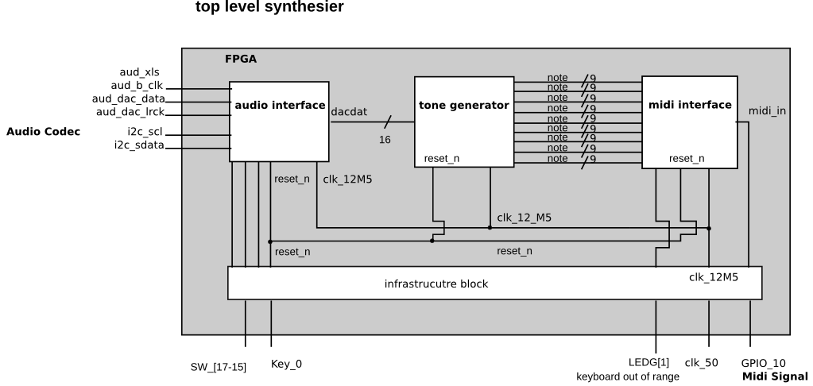
\includegraphics[width=0.9\textwidth]{images/midi_interface/top_synthesizer_block_saled.png}
	\caption{Top Synthesizer mit MIDI Interface: Blockschaltbild}
	\label{fig.top_synthesizer_block}
\end{figure}

Hier ist das Konzept der Umsetzung des MIDI Interface detaillierter beschrieben:

\begin{figure}[H]
	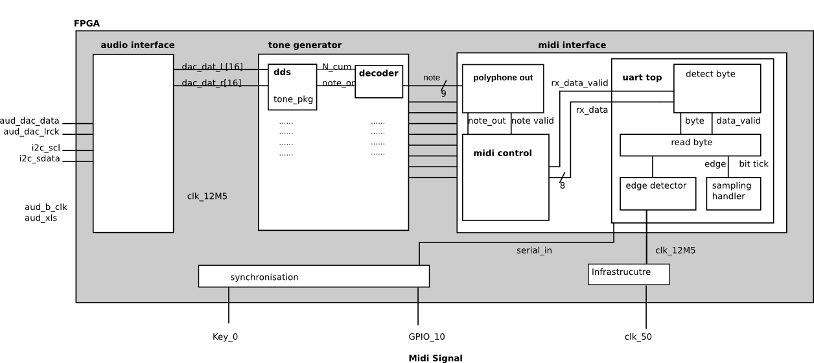
\includegraphics[width=0.9\textwidth]{images/midi_interface/top_synthesizer_detail_scaled.png}
	\caption{Top Synthesizer mit MIDI Interface: Detailansicht}
	\label{fig.top_synthesizer_detail}
\end{figure}

\chapter{RTL Top-Synthesizer}\label{chap.anhang_rtl_top_synthesizer}

\begin{figure}[H]
	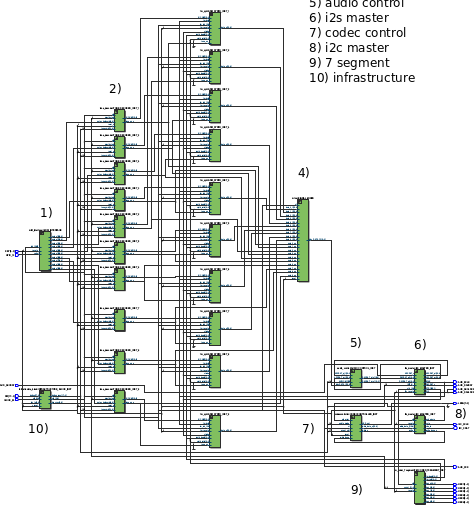
\includegraphics[width=0.9\textwidth]{images/midi_interface/RTL_10_Decoder_Mixwer.png}
	\caption{RTL Synthesizer-Projekt}
	\label{fig.rtl_top_synthesizer}
\end{figure}

	
	
	% add Bibliography to TOC
	\addcontentsline{toc}{chapter}{\bibname}              
	\bibliographystyle{IEEEtran}
	\bibliography{BibTex/references}

\end{document}
%---------------------------------------------------------------------
